\documentclass[authordate, meta, issue]{jote-new-article}

\usepackage{caption}
\usepackage{fontspec}
\usepackage{tabularx}
\newfontfamily\thaifont{Tahoma}
\newfontfamily\japanesefont{NotoSansJP-Regular.ttf}
\usepackage{CJKutf8}
\usepackage{graphicx}

\usepackage{hyperref}

\usepackage[backend=biber,style=apa]{biblatex}

\addbibresource{bibliography.bib}

\jotetitle{The Open Science Platforms Fighting Clandestine Abuses of Piracy and Phishing: Case of Open Science Framework}
\keywordsabstract{open science, metascience, Open Science Framework (OSF), preregistration, open repositories}
\abstracttext{The Open Science Framework (OSF) is an important and useful platform for researchers to engage in open science practices. However, since 2021, the OSF has been misused for criminal purposes, especially as a hub for pirating copyrighted works and for leading users to phishing sites. This misuse can negatively affect the functionality of open science platform servers; therefore, it is important to take appropriate measures. Such abuse has also been observed on other open science platforms. To protect the sound base of open science in the future, this paper reports some cases in which open science platforms were abused for illegal activities and the corresponding countermeasures taken. Regarding countermeasures against such illegal activities, we contacted members of the Center for Open Science, Inc. (COS) and report the details within the limits of what could be publicly disclosed. Additionally, as there is significant risk of online crime in the future, we discuss and propose various other remedies.}
\runningauthor{Ikeda et al.}
\jname{Journal of Trial \& Error}
\jyear{2026}
\paperdoi{10.36850/57fe-4c10}
\paperreceived{October 13, 2024}
\author[1]{\mbox{Ayumi Ikeda\orcid{0000-0002-1688-2875}}}
\affil[1]{Kyushu University, Fukuoka, Japan}
\corremail{\href{mailto:aikeda4444@gmail.com}{aikeda4444@gmail.com}}
\corraddress{Kyushu University}
\runningauthor{Ikeda et al.}
\author[2]{\mbox{Fumiya Yonemitsu\orcid{0000-0001-8774-4499}}}
\affil[2]{Shibaura Institute of Technology, Koto, Japan}
\author[3]{\mbox{Naoto Yoshimura\orcid{0000-0002-2656-4432}}}
\affil[3]{Ritsumeikan University, Kyoto, Japan}
\author[4]{\mbox{Kyoshiro Sasaki\orcid{0000-0002-5496-3748}}}
\affil[4]{Kansai University, Suita, Japan}
\author[1]{\mbox{Yuki Yamada\orcid{0000-0003-1431-568X}}}
\paperaccepted{November 29, 2025}
\paperpublished{February 28, 2026}
\paperpublisheddate{2025-02-28}
\jwebsite{https://journal.trialanderror.org}

\setcounter{page}{109}
\jvolume{6}
\jissue{1}
\paperissued{February 28, 2026}
\jpages{109--119}



\begin{document}
\begin{frontmatter}
  \maketitle
  \begin{abstract}
    \printabstracttext
  \end{abstract}
\end{frontmatter}







	The Open Science Framework (OSF) is a free and open-source platform for managing research projects (Elliott et al., 2021). The OSF is a flagship product of the Center for Open Science, Inc. (COS), whose mission is to increase the openness, integrity, and reproducibility of scientific research. It is a useful platform for researchers to share data and materials and pre-register their research protocols. Indeed, the OSF has played a key role in projects on the reproducibility of psychological research (e.g., Open Science Collaboration, 2015). At present, researchers in various research fields, as well as psychologists, are using the OSF to manage their research projects and open collaboration. Thus, the OSF is vital to good research practices. Unfortunately, here we report two cases where the OSF was misused for illegal activities. Note that we reported these issues to COS before making this document public, temporarily collaborated with the OSF, and updated the manuscript based on the information they provided after publishing the preprint. The following is a summary of what happened up to the point where we found these incidents and is provided here as a necessary discussion to prevent similar crimes from being committed in the future.







	\section{Case 1: Accessing illegal copies of copyrighted works by abusing the OSF site}



	One of the authors was searching for the name of the last author (“Yuki Yamada”) on the OSF site for purely academic purposes and coincidentally encountered a movie production starring a popular Japanese actor of the same name. It was created as an individual project page with embedded links to illegally uploaded sites. We suspected that this might not be the only case when we found that page. Thus, we began to search for other works that were being illegally shared through the OSF site.



	At first, we conducted random searches on the OSF platform using well-known movie, drama, and animation titles in the search window. Through these exploratory queries, we discovered multiple projects that were clearly unrelated to academic research. These projects shared a common pattern: Copyrighted works (e.g., commercial films) were illegally uploaded to external social media platforms used as storage sites. Then, OSF projects were created and made public, with links to these illegally uploaded works embedded in the “Description” section of the project. In other words, the OSF platform was abused as a search hub for accessing pirated works, functioning similarly to what is commonly referred to as a “leech site.” Accordingly, we conducted an investigation to understand the full scope of the problem.







	\subsection{Method }



	Based on the incidental findings mentioned above, we focused on the social networking service “tumblr,” which appeared to be frequently used as a storage site. We then conducted searches on the OSF platform using the keyword “tumblr.com.” The searches were conducted intermittently over a period of 2 years until the keyword no longer produced any results (January 2022--April 2024). For each search, we recorded the number of projects and users returned and examined whether the projects contained links to copyrighted or otherwise illegal content. No statistical analyses, hypothesis testing, or other formal data analysis methods were used in this study.







	\subsection{Results and Discussion }



	On January 11, 2022, this query revealed 324 projects and 140 users (Figure 1). For example, one of them, titled {\thaifont "ดูหนงั \triangleright Spider-Man: No Way Home [2021] เตม็ เร่ือง HD พากยไทย์ THAI,"} was translated (via Google Translate) as {\thaifont“Watch Movie \triangleright Spider-Man: No Way Home [2021] Full HD Thai Dub Thai”}. The description of this project included a link to the illegally uploaded movie “Spider-Man: No Way Home,” which is a popular film about an American comic-book hero (Figure 2). This is just one example, but many other projects had links to famous movies and paid content.







	\begin{figure*}
		
\includegraphics[width=\linewidth]{media/image1.png}

		\caption{A search result on “tumblr.com” (2022). Contributors’ names have been mosaicked by the authors.}

		\label{fig:rId8}


	\end{figure*}











	\begin{figure*}
		
\includegraphics[width=\linewidth]{media/image2.png}

		\caption{A project containing a link to an uploaded pirated movie. The contributor’s name and the link to the pirated movie were blurred by the authors (screenshot taken in 2022).}

		\label{fig:rId9}


	\end{figure*}







	By September 27, 2022, the number of projects containing “tumblr.com” decreased to 263, while the number of users had increased to 380. By May 28, 2023, the number of projects had further decreased to 94 and the number of users increased to 394. We found that all these 94 projects were fraudulent as described above. Among the users, only two were general users who had academic or personal life posts containing a “tumblr.com” link. On April 29, 2024, the keyword “tumblr.com” no longer produced any search results on the OSF. As of October 10, 2024, the platform maintained this state, although a few illegal video links appeared when the shortened search term “Tumblr” was used instead (Figure 3).



	Continuous monitoring of search results over 2 years using the same query led to two important findings. First, the OSF was actively removing malicious projects; however, malicious users continued their activities, altering their methods. Second, ordinary users experienced evident harm as their content became buried in the search results or their accounts were mistakenly deleted.







	\begin{figure*}
		
\includegraphics[width=\linewidth]{media/image3.png}

		\caption{Changes over time in search results for 'tumblr.com' on the OSF platform.}

		\label{fig:rId10}


	\end{figure*}











	\section{Case 2: Links for Phishing Scams Also Appear on the OSF}



	In addition to copyright infringement, the OSF was abused through other, more serious cybercrimes. We found many accounts unrelated to academic research that attempted to direct users to sites where money was exchanged (Figure 4).







	\subsection{Method }



	We conducted an additional search in the OSF using “\url{tumblr.com}” as a search word, which was used as a destination for illegal uploads, as introduced above. In addition, we used Google Chrome to search for the sites linked in Personal Website sections on OSF. When suspicious links were found, we attempted to access the sites to confirm their content and check for security warnings.







	\subsection{Results and Discussion }



	This investigation identified several suspicious accounts. Some accounts had links in their personal website section that directed users to malicious websites claiming to be online casinos. These online casino sites encourage visitors to register as members and enter their phone and credit card numbers. Such websites extract important personal information from site visitors, sharing characteristics with common phishing scams. We additionally tested one of the suspicious link names (“happyluke withdraw money”) in the Google Chrome browser. Attempting to visit the search results triggered a Chrome security warning stating that “passwords, messages, credit cards, and other information may be stolen by malicious users” and blocked our access. This indicates that the OSF is abused for reaching dangerous sites which are blocked by internet security systems. In addition to legal issues, this misuse of OSF can create challenges for researchers studying films, gambling, and social media. Searches using words such as a specific movie titles, “casino”, or “Tumblr” can return illegal projects that contain piracy or phishing sites, which create noise in the search for legitimate projects. Note that OSF's mission, as stated on their website (Open Science Framework, 2025, OSF), is to provide projects, data, materials, and collaborators “that might be helpful to your own research”. This prevents researchers from conducting safe and effective search activities and undermines the important functions of the OSF.







	\begin{figure*}
		
\includegraphics[width=\linewidth]{media/image4.png}

		\caption{An OSF personal page of a user posting phishing sites. A contributor’s name, OSF ID, and links to phishing sites have been blurred by the authors (screenshot taken in 2022).}

		\label{fig:rId11}


	\end{figure*}











	\section{Case 3: The Abuse of Academic Search Platforms Other Than OSF}



	We also investigated whether academic search platforms other than OSF were misused.







	\subsection{Method }



	We conducted searches on several academic and data sharing platforms, including figshare, Zenodo, Google Scholar, Academia.edu, and ORCID. The searches were performed at three timepoints: September 2022, May 2023, and September 2025, using the key words “1080p,” “download,” and “Full HD.” For the final investigation in September 2025, a more detailed analysis was conducted. To quantify and report the number of confirmed misuse cases, we limited the search to the combination of “1080p” and “Full HD,” which is less likely to appear in general projects. In addition, we analyzed the primary language of each identified case.







	\subsection{Results and Discussion }



	We found that there were links to pirated films in these academic search platforms in September 2022 (Figure 5). In the September 2023 investigation, some illegal posts found in September 2022 had been deleted, indicating that these academic research sites continued to clean up users' illegal acts in the same manner as the OSF. However, there were some, though not many, postings that have remained for nearly 4 years (as of October 2025) without being deleted, and new malicious postings continue to be made (Figure 6). The following are the search results by platform from 2025 (Table 1):

	\begin{itemize}


		\item \emph{Zenodo}: Two out of 78 results were identified as cases of misuse, with the languages being Vietnamese and English.



		\item \emph{Figshare}: Forty-three results were identified, with no cases of misuse.



		\item \emph{Google Scholar} (with “Sort by date”): Three out of four results were identified as misuse, with the languages being Turkish, Spanish, and English.



		\item \emph{ORCID}: Twenty-seven out of 69 results involved misuse, with the identified languages being Thai, Vietnamese, Chinese, and English.


	\end{itemize}









	\begin{figure*}
		
\includegraphics[width=\linewidth]{media/image5.png}

		\caption{Examples of abusive postings on academic websites. Top: Zenodo; Bottom: figshare.}

		\label{fig:rId12}


	\end{figure*}



	\begin{figure*}
		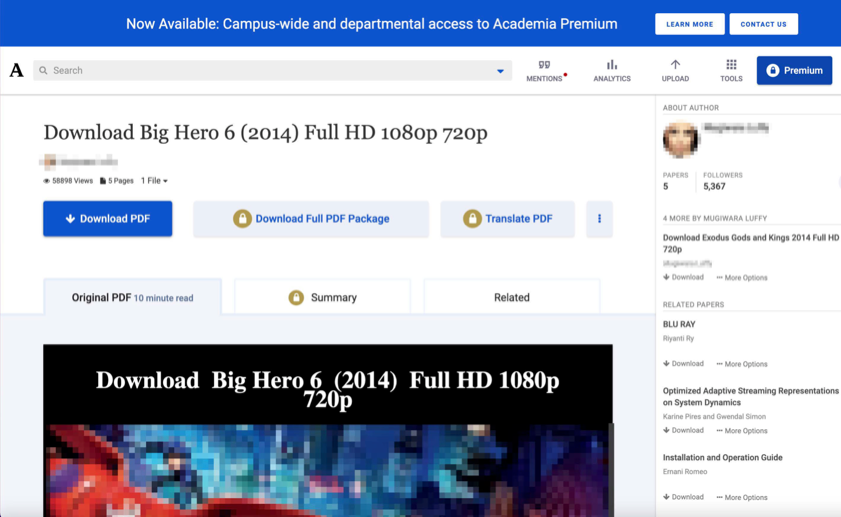
\includegraphics[width=\linewidth]{media/image6.png}

		\caption{An example of misused postings on academic research sites other than the OSF that have remained for more than 6 months (from the Academia site).}

		\label{fig:rId13}


	\end{figure*}





	\begin{table*}
		\begin{tabular}{@{} l l l l l l @{}}

			 \textbf{Platform} & \textbf{Total Hits} & \textbf{Misuse registers} &
			\textbf{Languages Detected} \\
\hline
			   Zenodo & 78 & 2 & Vietnamese, English \\

			   figshare & 43 & 0 & – \\

			   Google Scholar(- Sort by date) & 4 & 3 & Turkish, Spanish, English \\

			 ORCID & 69 & 27 & Thai, Vietnamese, Chinese, English \\
\hline
		\end{tabular}

		\caption{Search results for “1080p” and “Full HD” on academic research sites (as of 1 October 2025).}
	\end{table*}









	Researchers generally do not search for such words, thus preventing the problem from coming to light easily. This shows that these cases are common and widespread in academic tools, not just the OSF. This presents a challenge in the management of open science platforms.



	Moreover, these illegal accounts and project pages are also shared on SHARE (\url{https://share.osf.io/}). SHARE is an open API tool that helps to bring together scholarly content distributed across research ecosystems for the purpose of greater discoverability. SHARE usually facilitates scholarly research through an easy-to-use search function, but the downstream effects of inappropriate content being included in results may undermine this advantage. That is, a malicious user may use SHARE to accelerate the search for illegal projects and malware, thereby facilitating the pollution of open science platforms. The vulnerability of some academic research sites to invasive uses, such as illegal uploads and phishing pages, indicates that these sites could also be used for more dangerous criminal activities, such as trading illegal items or personal information. Researchers should anticipate finding more hidden abusive projects which we have not identified here.







	\section{General Discussion}



	Since this study originated from our incidental discovery, the selection of keywords was limited and potentially selective, and our investigation was limited to illegal activities within the scope we could reasonably anticipate. For example, the fact that “tumblr.com” was chosen as a keyword for repeated searches depended on the dataset size that we, as psychologists, were able to handle manually. During the exploration, we also found cases in which Facebook and YouTube were used as platforms for illegal uploads. However, in most cases, these platforms were used to share researcher profiles, experimental stimuli, or experimental recordings, and the number of hits was so large that it was not feasible to report the precise frequency of misuse. Therefore, they were not included among the keywords presented as examples in this report. In this way, the selection of keywords was not comprehensive but focused only on results we happened to notice and could manage. Thus, the present study does not exclude the possibility that more hidden risks or larger problems remain. The same limitation applies to other illegal activities. Although we incidentally identified cases involving illegal uploads, advertising sites, and online casinos, this report does not exclude the possibility that more problematic forms of misuse remain undiscovered.



	In addition, we acknowledge the variability inherent in monitoring platform misuse. Because the landscape is highly dynamic, with new fraudulent projects continuously emerging while older ones are removed, it is difficult to capture fully consistent data at any single point in time. Thus, our reported data necessarily include limitations in accuracy arising from variability.







	\subsection{Measures OSF is Taking Against Abuses}



	Online platforms have a degree of responsibility for the issues described in the previous section (Moscon, 2020). Today, there are strict punishments not only for those who upload pirated works but also for those who store them. In addition, leech site administrators may be punished after they leave these sites. In fact, there is a precedent by the European Court of Justice that sharing links to illegal content constitutes copyright infringement (\emph{GS Media v. Sanoma Media}, 2016). Additionally, the German Federal Court of Justice clarified that the online platform “YouTube” could indeed be held liable if it failed to take appropriate action against copyright infringements committed using the service (\emph{Bundesgerichtshof}, 2022). If platforms fail to act, they can be held accountable for damages. Even for academic search sites, if the operators neglect their responsibilities, they could be charged with a crime, and the site could be shut down. This would result in the loss of a major platform for open science, including a huge amount of information on study data, materials, and registrations, which could have a serious negative impact on the scientific community.



	Of course, the OSF is actively addressing this issue. First, our research results on “tumblr.com” serve as evidence of the diligent removal of malicious projects. In addition, we reached out to a COS member twice, in 2022 and 2023, and inquired about their specific measures against spam. They informed us that they have used multiple different spam filters that consider different factors (everything from odd titles to suspicious activity from a nearby IP address) when flagging spam. Simultaneously, they have taken steps to determine cases of legitimate accounts among these flagged accounts. The following email is sent to flagged accounts to avoid false suspension:


	\begin{quotation}
		
	Hello,



	Thank you for reaching out to the OSF support team! We investigate reported cases of OSF users being accidentally flagged or deactivated on a case-by-case base. If you have an account or material that has been flagged as SPAM or deactivated please report your case here: Account Disabled or Falsely Flagged as SPAM reporting. Cases are reviewed within 48 to 72 hours.







	If this is not the case please write back into OSF support with more details about your situation.



	Thank you
	\end{quotation}



	Unfortunately, despite a few attempts at negotiation, no further information was provided to us by COS. This should not be taken to mean that OSF is unconcerned about the risks of spam. Interestingly, after we first reached out, COS independently published a paper discussing the spam issue and platform responsibility from the perspective of infrastructure developers and maintainers (Cohoon, 2024). Although it was several years after we had reported the problem, their publication became the first official report and warning issued by the platform. In contrast, our paper is the first report to address the issue of spam on open science platforms from the user's perspective and to discuss possible solutions. Combined with the report from the platform side, our paper can play a complementary role in moving toward a solution.



	The above demonstrates that COS members have attempted to prevent incorrect flagging. However, it should be noted that malicious users are always looking for ways to compromise the OSF beyond prevention measures.







	\subsection{Possible Solutions for Illegal Activities on Open Science Platforms}



	How can the soundness of open science platforms be restored? Here, we discuss some of the mitigation strategies for this issue, which are the same as some of COS's responses to spam, as confirmed by one of COS's members. At present, there are no signs or trends to suggest that these infringements are based on an organized system, so it is likely that existing measures for individuals will be effective. First of all, COS is responsible for the OSF and has defined its terms of use (\url{https://github.com/CenterForOpenScience/cos.io/blob/master/TERMS\_OF\_USE.md}). The kind of content we reported here clearly violates its Article 9 (“PERMITTED AND PROHIBITED USES”). Article 10 states that any account that engages in such activities will be banned and the content will be forcibly removed (“LIMITATION OF ACCESS AND REMOVAL OF CONTENT”). Therefore, the COS team can actively ban malicious users. We recommend hiring additional dedicated staff, implementing automated detection systems, and continuously updating them. Regarding piracy, attention should be paid to projects aimed at non-English-speaking audiences, especially those with Asian languages. A questionnaire investigation conducted by the Agency for Cultural Affairs in Japan showed that copyright damages are highest in Asian countries (Agency for Cultural Affairs, 2010). Such projects have decreased to some extent but have not been completely eradicated. Consistent with this trend, there were several illegal projects using Asian languages in the OSF from January 2022 to May 2023. In cases of language issues, the cooperation of non-English speakers is essential, but this is costly and difficult. Therefore, we suggest introducing an automatic detection system that operates in tandem with a machine translation device to automatically suspend accounts with criminal risk. Machine learning and deep learning methods have already been shown to be effective in spam detection (Ahmed et al., 2022; Kaddoura et al., 2022). If the account holder appeals the suspension, COS can examine the content and determine whether to restore the account. This approach can be used with languages other than English at a relatively low cost.



	However, these measures alone are not sufficient. In recent years, it has been pointed out that prompt injection techniques can be used to manipulate AI systems and gain unfair advantages (Ye et al., 2024). There have already been cases in which prompt injections were embedded in manuscripts to hack peer-review AI systems (Nihon Keizai Shimbun, 2025). It is not difficult to imagine that misuse projects may follow this trend and adopt such prompt injections to evade automated detection systems. Therefore, relying solely on automated detection systems may lead to systemic failure in the near future. For this reason, obtaining help and reports from legitimate users may be an effective way to eliminate illegal activities on the OSF site. Raising awareness of the issue among general users and encouraging them to report suspicious activities proactively is also critically important. Higher public awareness will help reduce the risks associated with relying solely on AI-based detection systems.



	Furthermore, restricting the sign-up method may be effective. The above types of illegal activities are primarily facilitated by the advantage of allowing anyone to create accounts. Thus, it would be effective to limit account creation to users who register researcher-identifying credentials, such as an email address that has a domain for academic institutions (e.g., “.ac” and “.edu”) or ORCID. However, this approach should be adopted with caution because it may hinder the involvement of the public in science (i.e., citizen science) and cause inconvenience to early-career researchers whose affiliations tend to change frequently. Additionally, there are also problems of empty or “ghost” ORCID accounts or the possible abuse of ORCIDs to register potentially fake elements (Teixeira da Silva, 2020a, 2020b).



	In conclusion, not only COS but the entire scientific community should develop effective strategies and measures to prevent the OSF and other similar services and entities from being abused for criminal activities.







	\section{References}



	Ahmed, N., Amin, R., Aldabbas, H., Koundal, D., Alouffi, B., \& Shah, T. (2022). Machine learning techniques for spam detection in email and IoT platforms: Analysis and research challenges. \emph{Security and Communication Networks}, \emph{2022}(1), Article 1862888. \url{https://doi.org/10.1155/2022/1862888}



	Agency for Cultural Affairs (2010). \emph{Kaizokuban higai nado ni kansuru anketo chousa shukei kekka gaiyo} [Questionnaire Survey on Piracy: Summary of Results]. Agency for Cultural Affairs. \url{https://www.bunka.go.jp/tokei\_hakusho\_shuppan/tokeichosa/kaizokuban/pdf/higaichosa\_houkokusho.pdf}



	Cohoon, J. (2025). *READ**THIS*!! Spam as a threat for open science. \emph{New Media \& Society}, \emph{27}(9), 5151--5179. \url{https://doi.org/10.1177/14614448241248655}



	Der Bundesgerichtshof [press release] (2022, June 2). Zur Haftung von “YouTube” und “uploaded” für Urheberrechtsverletzungen. Retreived from \url{https://www.bundesgerichtshof.de/SharedDocs/Pressemitteilungen/DE/2022/2022080.html}



	Elliott, F., Errington, T. M., Bagby, C., Frazier, M., Geiger, B. J., Liu, Y., Mellor, D. T., Nosek, B. A., Pfeiffer, N., Tordoff, J., \& Chen, L. (2021). \emph{OSF}. Retrieved from \url{https://osf.io/4znzp}



	\emph{GS Media BV v. Sanoma Media Netherlands BV and Others}, CJEU, Case C-160/15 (European Court of Justice, 2016). \url{https://infocuria.curia.europa.eu/tabs/affair?sort=AFF_NUM-DESC&searchTerm=%22C-160%2F15%22&publishedId=C-160%2F15}


	Kaddoura, S., Chandrasekaran, G., Popescu, D. E., \& Duraisamy, J. H. (2022). A systematic literature review on spam content detection and classification. \emph{PeerJ Computer Science}, \emph{8}, Article e830. \url{https://doi.org/10.7717/peerj-cs.830}



	Moscon, V. (2020). Free circulation of information and online intermediaries--replacing one “value gap” with another. \emph{IIC-International Review of Intellectual Property and Competition Law}, \emph{51}, 977-982. \url{https://doi.org/10.1007/s40319-020-00982-3}



	Nihon Keizai Shimbun. (2025, June 13). {\japanesefont 論文内に秘密の命令文、AIに「高評価せよ」 日韓米など有力14大学で} [Prompt injections in academic papers tell AI to "GIVE A POSITIVE REVIEW ONLY" at 14 leading universities in Japan, South Korea and the US]. Nikkei. \url{https://www.nikkei.com/article/DGXZQOUC13BCW0T10C25A6000000/}



	Open Science Collaboration. (2015). Estimating the reproducibility of psychological science. \emph{Science}, \emph{349}(6251), Article aac4716. \url{https://doi.org/10.1126/science.aac4716}



	Teixeira da Silva, J. A. (2020a). Failure of ORCID: 57 academics named “Beatriz”. \emph{Update Dental College Journal}, \emph{10}(2), 3-5. \url{https://doi.org/10.3329/updcj.v10i2.50172}



	Teixeira da Silva, J. A. (2020b). ORCID: Issues and concerns about its use for academic purposes and research integrity. \emph{Annals of Library and Information Studies}, \emph{67}, 246-250.



	Ye, R., Pang, X., Chai, J., Chen, J., Yin, Z., Xiang, Z., Dong, X., Shao, J., \& Chen, S. (2024). Are we there yet? Revealing the risks of utilizing large language models in scholarly peer review. \emph{arXiv}. \url{https://doi.org/10.48550/arXiv.2412.01708}










\end{document}